\documentclass[conference]{IEEEtran}

\usepackage{draftwatermark}
\usepackage[backend=bibtex]{biblatex}

\addbibresource{report.bib}
\nocite{*}

\begin{document}

	\title{Lag compensation techniques for networked games}
	\author{\IEEEauthorblockN{James Robinson}
	\IEEEauthorblockA{Electronics and Computer Science\\
	University of Southampton\\
	Email: jr4e09@soton.ac.uk}}
	\maketitle

	\begin{abstract}
		In networked multiplayer games, network latency often introduces an unacceptable delay between when the player attempts to take an action and when the action actually takes effect within the game world. In this paper, methods of quantifying the effects of this latency, algorithms that mask its apparent effects, and a selection of novel unified frameworks for lag compensation are explored. Also discussed are the advantages and limitations of each algorithm, along with their potential applications.
	\end{abstract}

	\section{Introduction}

	% Explain what kinds of games we're talking about and general terminology
	% Assume tick-based games

	In gaming, the term ``lag'' refers to the delay between when the user takes an action, and when the action takes effect within the game world. Lag can be introduced by many factors including input device latency, framerate, vsync, and monitor response time, but the most egregious source of lag in networked or online games is the latency between client and server. Although techniques exist to reduce this latency, the fact that data transfer is limited by the speed of light means that this latency can never be completely eliminated.

	Lag reduces player engagement and enjoyment, and furthermore can impact performance in competitive multiplayer games \cite{beigbeder2004effects}. For this reason, most popular online games take measures to reduce the effect of network latency on the player's experience. Such techniques are generally referred to as ``lag compensation'' algorithms. Many such techniques exist, each of which make various tradeoffs that are appropriate for some types of game. Because of the disparate requirements of different genres of game, no ``silver bullet'' solution exists.

	In this paper, I will introduce various state of the art techniques for lag compensation in networked multiplayer games, discussing their advantages and disadvantages, as well as which types of simulation each technique is suited to. I will also present some unified models.

	\section{Quantifying effects of latency}

	TODO \cite{beigbeder2004effects} \cite{chen2011perceptual} \cite{claypool2005effect} \cite{fritsch2005effect} \cite{sheldon2003effect} \cite{quax2004objective} \cite{dick2005analysis}

	\section{Methods of lag compensation}

	\subsection{Client-side}

	\subsubsection{Extrapolation (``dead reckoning'')}

	The simplest form of client-side lag compensation is ``dead reckoning'' (named for the principle used in navigation). Under this approach, the last known positions and velocities of each game object are used to predict their current position via extrapolation, taking latency into account. For example, given current time $t$, current latency $l$, and a game object with last known position $\hat{s}_{t - l}$ and velocity $\hat{v}_{t - l}$, the predicted position at the current point in time is $\hat{s}_{t} = \hat{s}_{t - l} + l\hat{v}_{t - l}$. Figure~\ref{fig:extrapolation_timeline} shows a timeline of this approach: updates from the server take some amount of time to reach the client, and the client extrapolates game object positions to predict where they are now.

	\begin{figure}
		\centering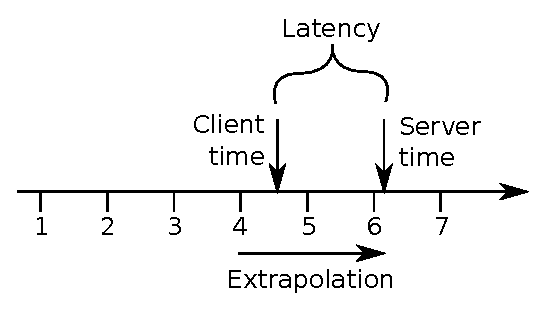
\includegraphics[width=\linewidth]{figures/extrapolation_timeline.eps}
		\caption{A timeline showing extrapolation}
		\label{fig:extrapolation_timeline}
	\end{figure}

	Misprediction errors are very common under this scheme, occurring every time the velocity or bearing of a game object changes. The simplest way to correct misprediction errors is to immediately ``snap'' the object to the correct location once an update arrives from the server, but this can cause very visible visual discontinuities that can be distracting for the player. A less accurate but visually smoother approach is to interpolate between the position that the entity was last rendered at and its current estimated position (as shown in figure~\ref{fig:extrapolation}). This smooths out the visual discontinuities but also further reduces precision.

	\begin{figure}
		\centering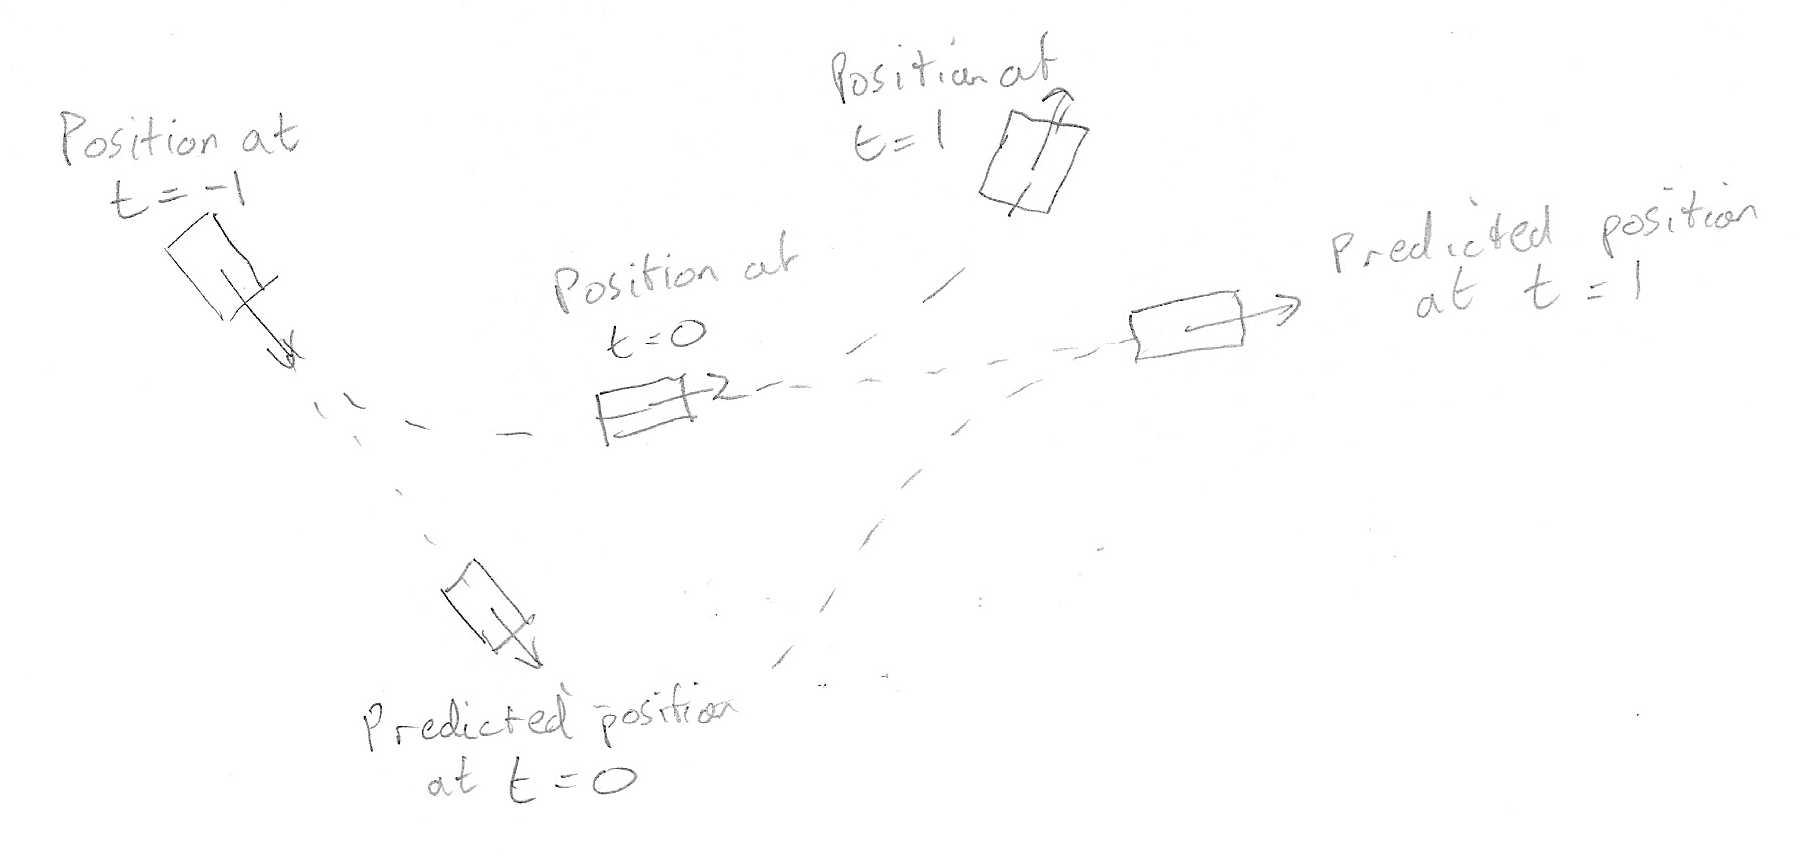
\includegraphics[width=\linewidth]{figures/extrapolation.jpg}
		\caption{Misprediction}
		\label{fig:extrapolation}
	\end{figure}

	It is important to note that when using this scheme, game objects are very rarely (if ever) rendered at correct, accurate positions. This tradeoff is acceptable for some games, particularly where game objects change velocity or bearing reasonably slowly (for example, cars in a racing game) \cite{pantel2002suitability}, but for games requiring pinpoint accuracy, a better scheme is required.

	\subsubsection{Interpolation}

	An alternative approach to client-side lag compensation is to buffer updates received from the server for some time before rendering them. By doing this, the client can ensure that it always has at least two ``real'' world states between which it can interpolate, which completely eliminates the misprediction errors mentioned previously. A timeline showing this approach is given in figure~\ref{fig:interpolation_timeline}. Note that because the client buffers 3 updates, this system is also tolerant of occasional packet loss; the client always has at least 2 snapshots to interpolate between, even if 1 packet goes missing.

	An immediately apparent problem with this approach is that while reducing the apparent effects of latency, it actually \emph{induces} additional latency by virtue of ``queuing up'' updates before they are rendered. Thus prediction must be applied to the game object controlled by the player in order to maintain interactivity.

	If the client runs out of buffered packets (due to packet loss or server error), it may either freeze until a new state is received, or fall back to extrapolation. In the latter case, the same disadvantages detailed in the previous section occur.

	\begin{figure}
		\centering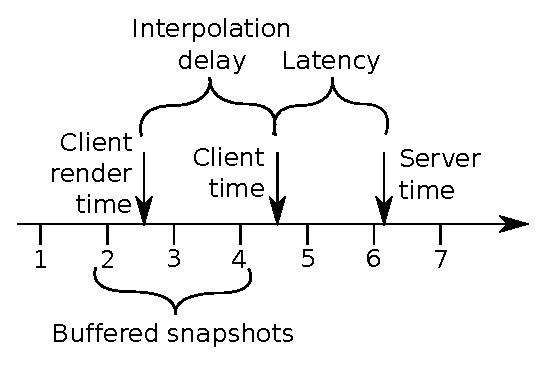
\includegraphics[width=\linewidth]{figures/interpolation_timeline.eps}
		\caption{A timeline showing the latency between client and server, and the delay introduced by interpolation of buffered world states.}
		\label{fig:interpolation_timeline}
	\end{figure}

	\subsection{Server-side}

	\subsubsection{No compensation}

	The simplest approach to server-side lag compensation is to do nothing at all. If the clients are already predicting future world states via extrapolation, then the server doesn't need to do anything. If the clients are \emph{not} predicting future world states (for example, if they follow the buffering/interpolation approach detailed above), then a consequence of not applying server-side lag compensation is that players must lead their targets by an amount proportional to their latency and (if applicable) the interpolation period.

	\subsubsection{Authoritative clients}

	Another very simple approach is to make clients authoritative over their actions. For example, if the client says ``I am now at position X and I have killed player Y'', the server will just blindly accept this new information, move the player to position X, and mark player Y as dead. This only works if all clients can be trusted, which immediately rules out most real-world scenarios due to the possibility of cheating.

	\subsubsection{Buffering of world state}

	\cite{bernier2001latency}

	\begin{itemize}
		\item Buffer 1 sec of previous world states
		\item When a client command arrives, rewind time based on their latency and (if applicable) their interp amount, interpolating between wold states if the command occurred between ticks
		\item Execute the command in the context of this world state
		\item This can cause temporal paradoxes - players can be shot after they duck behind cover. Usually a tradeoff the developer is willing to make since it ensures responsiveness for all players
		\item If player latency varies too much (for example, if data follows many different routes), this is inaccurate. Works best if constant latency can be guaranteed
		\item Gives ``peek advantage'' when players go round corners, more pronounced if there is a large latency difference between the players in the exchange
	\end{itemize}

	\subsection{Network-level}

	TODO \cite{yu2008latency} \cite{yu2012latency}

	\section{Supporting technologies}

	\subsection{Clock synchronisation}

	TODO \cite{cristian1989probabilistic}

	\subsection{Delta encoding}

	No sources found yet, other than Quake 3 source code

	\section{Unified frameworks}

	TODO \cite{savery2013timelines} \cite{touch1992mirage} \cite{diot1999distributed}

	\section{Conclusions}

	TODO

	\printbibliography

\end{document}
